\documentclass[1p]{elsarticle_modified}
%\bibliographystyle{elsarticle-num}

%\usepackage[colorlinks]{hyperref}
%\usepackage{abbrmath_seonhwa} %\Abb, \Ascr, \Acal ,\Abf, \Afrak
\usepackage{amsfonts}
\usepackage{amssymb}
\usepackage{amsmath}
\usepackage{amsthm}
\usepackage{scalefnt}
\usepackage{amsbsy}
\usepackage{kotex}
\usepackage{caption}
\usepackage{subfig}
\usepackage{color}
\usepackage{graphicx}
\usepackage{xcolor} %% white, black, red, green, blue, cyan, magenta, yellow
\usepackage{float}
\usepackage{setspace}
\usepackage{hyperref}

\usepackage{tikz}
\usetikzlibrary{arrows}

\usepackage{multirow}
\usepackage{array} % fixed length table
\usepackage{hhline}

%%%%%%%%%%%%%%%%%%%%%
\makeatletter
\renewcommand*\env@matrix[1][\arraystretch]{%
	\edef\arraystretch{#1}%
	\hskip -\arraycolsep
	\let\@ifnextchar\new@ifnextchar
	\array{*\c@MaxMatrixCols c}}
\makeatother %https://tex.stackexchange.com/questions/14071/how-can-i-increase-the-line-spacing-in-a-matrix
%%%%%%%%%%%%%%%

\usepackage[normalem]{ulem}

\newcommand{\msout}[1]{\ifmmode\text{\sout{\ensuremath{#1}}}\else\sout{#1}\fi}
%SOURCE: \msout is \stkout macro in https://tex.stackexchange.com/questions/20609/strikeout-in-math-mode

\newcommand{\cancel}[1]{
	\ifmmode
	{\color{red}\msout{#1}}
	\else
	{\color{red}\sout{#1}}
	\fi
}

\newcommand{\add}[1]{
	{\color{blue}\uwave{#1}}
}

\newcommand{\replace}[2]{
	\ifmmode
	{\color{red}\msout{#1}}{\color{blue}\uwave{#2}}
	\else
	{\color{red}\sout{#1}}{\color{blue}\uwave{#2}}
	\fi
}

\newcommand{\Sol}{\mathcal{S}} %segment
\newcommand{\D}{D} %diagram
\newcommand{\A}{\mathcal{A}} %arc


%%%%%%%%%%%%%%%%%%%%%%%%%%%%%5 test

\def\sl{\operatorname{\textup{SL}}(2,\Cbb)}
\def\psl{\operatorname{\textup{PSL}}(2,\Cbb)}
\def\quan{\mkern 1mu \triangleright \mkern 1mu}

\theoremstyle{definition}
\newtheorem{thm}{Theorem}[section]
\newtheorem{prop}[thm]{Proposition}
\newtheorem{lem}[thm]{Lemma}
\newtheorem{ques}[thm]{Question}
\newtheorem{cor}[thm]{Corollary}
\newtheorem{defn}[thm]{Definition}
\newtheorem{exam}[thm]{Example}
\newtheorem{rmk}[thm]{Remark}
\newtheorem{alg}[thm]{Algorithm}

\newcommand{\I}{\sqrt{-1}}
\begin{document}

%\begin{frontmatter}
%
%\title{Boundary parabolic representations of knots up to 8 crossings}
%
%%% Group authors per affiliation:
%\author{Yunhi Cho} 
%\address{Department of Mathematics, University of Seoul, Seoul, Korea}
%\ead{yhcho@uos.ac.kr}
%
%
%\author{Seonhwa Kim} %\fnref{s_kim}}
%\address{Center for Geometry and Physics, Institute for Basic Science, Pohang, 37673, Korea}
%\ead{ryeona17@ibs.re.kr}
%
%\author{Hyuk Kim}
%\address{Department of Mathematical Sciences, Seoul National University, Seoul 08826, Korea}
%\ead{hyukkim@snu.ac.kr}
%
%\author{Seokbeom Yoon}
%\address{Department of Mathematical Sciences, Seoul National University, Seoul, 08826,  Korea}
%\ead{sbyoon15@snu.ac.kr}
%
%\begin{abstract}
%We find all boundary parabolic representation of knots up to 8 crossings.
%
%\end{abstract}
%\begin{keyword}
%    \MSC[2010] 57M25 
%\end{keyword}
%
%\end{frontmatter}

%\linenumbers
%\tableofcontents
%
\newcommand\colored[1]{\textcolor{white}{\rule[-0.35ex]{0.8em}{1.4ex}}\kern-0.8em\color{red} #1}%
%\newcommand\colored[1]{\textcolor{white}{ #1}\kern-2.17ex	\textcolor{white}{ #1}\kern-1.81ex	\textcolor{white}{ #1}\kern-2.15ex\color{red}#1	}

{\Large $\underline{12a_{0180}~(K12a_{0180})}$}

\setlength{\tabcolsep}{10pt}
\renewcommand{\arraystretch}{1.6}
\vspace{1cm}\begin{tabular}{m{100pt}>{\centering\arraybackslash}m{274pt}}
\multirow{5}{120pt}{
	\centering
	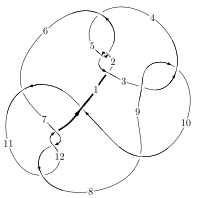
\includegraphics[width=112pt]{../../../GIT/diagram.site/Diagrams/png/981_12a_0180.png}\\
\ \ \ A knot diagram\footnotemark}&
\allowdisplaybreaks
\textbf{Linearized knot diagam} \\
\cline{2-2}
 &
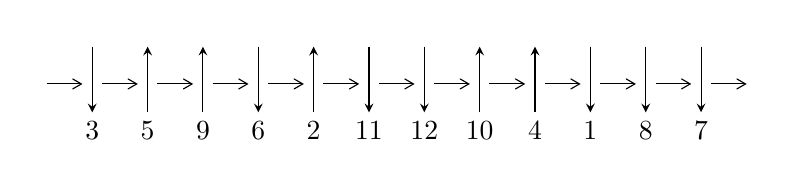
\begin{tikzpicture}[x=20pt, y=17pt]
	% nodes
	\node (C0) at (0, 0) {};
	\node (C1) at (1, 0) {};
	\node (C1U) at (1, +1) {};
	\node (C1D) at (1, -1) {3};

	\node (C2) at (2, 0) {};
	\node (C2U) at (2, +1) {};
	\node (C2D) at (2, -1) {5};

	\node (C3) at (3, 0) {};
	\node (C3U) at (3, +1) {};
	\node (C3D) at (3, -1) {9};

	\node (C4) at (4, 0) {};
	\node (C4U) at (4, +1) {};
	\node (C4D) at (4, -1) {6};

	\node (C5) at (5, 0) {};
	\node (C5U) at (5, +1) {};
	\node (C5D) at (5, -1) {2};

	\node (C6) at (6, 0) {};
	\node (C6U) at (6, +1) {};
	\node (C6D) at (6, -1) {11};

	\node (C7) at (7, 0) {};
	\node (C7U) at (7, +1) {};
	\node (C7D) at (7, -1) {12};

	\node (C8) at (8, 0) {};
	\node (C8U) at (8, +1) {};
	\node (C8D) at (8, -1) {10};

	\node (C9) at (9, 0) {};
	\node (C9U) at (9, +1) {};
	\node (C9D) at (9, -1) {4};

	\node (C10) at (10, 0) {};
	\node (C10U) at (10, +1) {};
	\node (C10D) at (10, -1) {1};

	\node (C11) at (11, 0) {};
	\node (C11U) at (11, +1) {};
	\node (C11D) at (11, -1) {8};

	\node (C12) at (12, 0) {};
	\node (C12U) at (12, +1) {};
	\node (C12D) at (12, -1) {7};
	\node (C13) at (13, 0) {};

	% arrows
	\draw[->,>={angle 60}]
	(C0) edge (C1) (C1) edge (C2) (C2) edge (C3) (C3) edge (C4) (C4) edge (C5) (C5) edge (C6) (C6) edge (C7) (C7) edge (C8) (C8) edge (C9) (C9) edge (C10) (C10) edge (C11) (C11) edge (C12) (C12) edge (C13) ;	\draw[->,>=stealth]
	(C1U) edge (C1D) (C2D) edge (C2U) (C3D) edge (C3U) (C4U) edge (C4D) (C5D) edge (C5U) (C6U) edge (C6D) (C7U) edge (C7D) (C8D) edge (C8U) (C9D) edge (C9U) (C10U) edge (C10D) (C11U) edge (C11D) (C12U) edge (C12D) ;
	\end{tikzpicture} \\
\hhline{~~} \\& 
\textbf{Solving Sequence} \\ \cline{2-2} 
 &
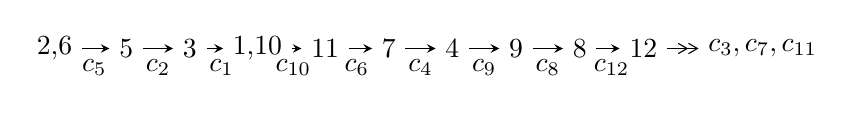
\begin{tikzpicture}[x=23pt, y=7pt]
	% node
	\node (A0) at (-1/8, 0) {2,6};
	\node (A1) at (1, 0) {5};
	\node (A2) at (2, 0) {3};
	\node (A3) at (49/16, 0) {1,10};
	\node (A4) at (33/8, 0) {11};
	\node (A5) at (41/8, 0) {7};
	\node (A6) at (49/8, 0) {4};
	\node (A7) at (57/8, 0) {9};
	\node (A8) at (65/8, 0) {8};
	\node (A9) at (73/8, 0) {12};
	\node (C1) at (1/2, -1) {$c_{5}$};
	\node (C2) at (3/2, -1) {$c_{2}$};
	\node (C3) at (5/2, -1) {$c_{1}$};
	\node (C4) at (29/8, -1) {$c_{10}$};
	\node (C5) at (37/8, -1) {$c_{6}$};
	\node (C6) at (45/8, -1) {$c_{4}$};
	\node (C7) at (53/8, -1) {$c_{9}$};
	\node (C8) at (61/8, -1) {$c_{8}$};
	\node (C9) at (69/8, -1) {$c_{12}$};
	\node (A10) at (11, 0) {$c_{3},c_{7},c_{11}$};

	% edge
	\draw[->,>=stealth]	
	(A0) edge (A1) (A1) edge (A2) (A2) edge (A3) (A3) edge (A4) (A4) edge (A5) (A5) edge (A6) (A6) edge (A7) (A7) edge (A8) (A8) edge (A9) ;
	\draw[->>,>={angle 60}]	
	(A9) edge (A10);
\end{tikzpicture} \\ 

\end{tabular} \\

\footnotetext{
The image of knot diagram is generated by the software ``\textbf{Draw programme}" developed by Andrew Bartholomew(\url{http://www.layer8.co.uk/maths/draw/index.htm\#Running-draw}), where we modified some parts for our purpose(\url{https://github.com/CATsTAILs/LinksPainter}).
}\phantom \\ \newline 
\centering \textbf{Ideals for irreducible components\footnotemark of $X_{\text{par}}$} 
 
\begin{align*}
I^u_{1}&=\langle 
40 u^{91}+119 u^{90}+\cdots+4 b+23,\;27 u^{91}+64 u^{90}+\cdots+4 a-3,\;u^{92}+4 u^{91}+\cdots+2 u+1\rangle \\
I^u_{2}&=\langle 
- a u+b,\;a^3- a^2 u+a^2+1,\;u^2- u+1\rangle \\
\\
\end{align*}
\raggedright * 2 irreducible components of $\dim_{\mathbb{C}}=0$, with total 98 representations.\\
\footnotetext{All coefficients of polynomials are rational numbers. But the coefficients are sometimes approximated in decimal forms when there is not enough margin.}
\newpage
\renewcommand{\arraystretch}{1}
\centering \section*{I. $I^u_{1}= \langle 40 u^{91}+119 u^{90}+\cdots+4 b+23,\;27 u^{91}+64 u^{90}+\cdots+4 a-3,\;u^{92}+4 u^{91}+\cdots+2 u+1 \rangle$}
\flushleft \textbf{(i) Arc colorings}\\
\begin{tabular}{m{7pt} m{180pt} m{7pt} m{180pt} }
\flushright $a_{2}=$&$\begin{pmatrix}0\\u\end{pmatrix}$ \\
\flushright $a_{6}=$&$\begin{pmatrix}1\\0\end{pmatrix}$ \\
\flushright $a_{5}=$&$\begin{pmatrix}1\\u^2\end{pmatrix}$ \\
\flushright $a_{3}=$&$\begin{pmatrix}u\\u^3+u\end{pmatrix}$ \\
\flushright $a_{1}=$&$\begin{pmatrix}u^3\\u^5+u^3+u\end{pmatrix}$ \\
\flushright $a_{10}=$&$\begin{pmatrix}-\frac{27}{4} u^{91}-16 u^{90}+\cdots-\frac{25}{2} u+\frac{3}{4}\\-10 u^{91}-\frac{119}{4} u^{90}+\cdots-\frac{53}{4} u-\frac{23}{4}\end{pmatrix}$ \\
\flushright $a_{11}=$&$\begin{pmatrix}-\frac{23}{4} u^{91}-\frac{57}{4} u^{90}+\cdots-\frac{45}{4} u+\frac{3}{2}\\-5 u^{91}-\frac{63}{4} u^{90}+\cdots-\frac{29}{4} u-\frac{19}{4}\end{pmatrix}$ \\
\flushright $a_{7}=$&$\begin{pmatrix}\frac{1}{4} u^{90}+\frac{3}{4} u^{89}+\cdots+\frac{17}{4} u+\frac{1}{4}\\-\frac{1}{4} u^{91}- u^{90}+\cdots+\frac{1}{2} u-\frac{1}{4}\end{pmatrix}$ \\
\flushright $a_{4}=$&$\begin{pmatrix}u^2+1\\u^2\end{pmatrix}$ \\
\flushright $a_{9}=$&$\begin{pmatrix}-\frac{25}{4} u^{91}-12 u^{90}+\cdots-\frac{17}{2} u+\frac{21}{4}\\-13 u^{91}-\frac{161}{4} u^{90}+\cdots-\frac{71}{4} u-\frac{25}{4}\end{pmatrix}$ \\
\flushright $a_{8}=$&$\begin{pmatrix}-\frac{9}{4} u^{91}-12 u^{90}+\cdots-\frac{27}{2} u-\frac{19}{4}\\-2 u^{91}-\frac{33}{4} u^{90}+\cdots-\frac{23}{4} u-\frac{21}{4}\end{pmatrix}$ \\
\flushright $a_{12}=$&$\begin{pmatrix}-\frac{7}{2} u^{91}-\frac{23}{2} u^{90}+\cdots-5 u-\frac{3}{2}\\\frac{5}{4} u^{91}+\frac{5}{4} u^{90}+\cdots+\frac{1}{4} u-\frac{5}{2}\end{pmatrix}$\\&\end{tabular}
\flushleft \textbf{(ii) Obstruction class $= -1$}\\~\\
\flushleft \textbf{(iii) Cusp Shapes $= -8 u^{91}-\frac{51}{2} u^{90}+\cdots-11 u-19$}\\~\\
\newpage\renewcommand{\arraystretch}{1}
\flushleft \textbf{(iv) u-Polynomials at the component}\newline \\
\begin{tabular}{m{50pt}|m{274pt}}
Crossings & \hspace{64pt}u-Polynomials at each crossing \\
\hline $$\begin{aligned}c_{1},c_{4}\end{aligned}$$&$\begin{aligned}
&u^{92}+32 u^{91}+\cdots+18 u+1
\end{aligned}$\\
\hline $$\begin{aligned}c_{2},c_{5}\end{aligned}$$&$\begin{aligned}
&u^{92}+4 u^{91}+\cdots+2 u+1
\end{aligned}$\\
\hline $$\begin{aligned}c_{3},c_{9}\end{aligned}$$&$\begin{aligned}
&u^{92}+u^{91}+\cdots+32 u+64
\end{aligned}$\\
\hline $$\begin{aligned}c_{6}\end{aligned}$$&$\begin{aligned}
&u^{92}+3 u^{91}+\cdots-3 u+1
\end{aligned}$\\
\hline $$\begin{aligned}c_{7},c_{11},c_{12}\end{aligned}$$&$\begin{aligned}
&u^{92}-3 u^{91}+\cdots-5 u+1
\end{aligned}$\\
\hline $$\begin{aligned}c_{8}\end{aligned}$$&$\begin{aligned}
&u^{92}-35 u^{91}+\cdots-70656 u+4096
\end{aligned}$\\
\hline $$\begin{aligned}c_{10}\end{aligned}$$&$\begin{aligned}
&u^{92}-21 u^{91}+\cdots-69583 u+3971
\end{aligned}$\\
\hline
\end{tabular}\\~\\
\newpage\renewcommand{\arraystretch}{1}
\flushleft \textbf{(v) Riley Polynomials at the component}\newline \\
\begin{tabular}{m{50pt}|m{274pt}}
Crossings & \hspace{64pt}Riley Polynomials at each crossing \\
\hline $$\begin{aligned}c_{1},c_{4}\end{aligned}$$&$\begin{aligned}
&y^{92}+60 y^{91}+\cdots+102 y+1
\end{aligned}$\\
\hline $$\begin{aligned}c_{2},c_{5}\end{aligned}$$&$\begin{aligned}
&y^{92}+32 y^{91}+\cdots+18 y+1
\end{aligned}$\\
\hline $$\begin{aligned}c_{3},c_{9}\end{aligned}$$&$\begin{aligned}
&y^{92}-35 y^{91}+\cdots-70656 y+4096
\end{aligned}$\\
\hline $$\begin{aligned}c_{6}\end{aligned}$$&$\begin{aligned}
&y^{92}- y^{91}+\cdots- y+1
\end{aligned}$\\
\hline $$\begin{aligned}c_{7},c_{11},c_{12}\end{aligned}$$&$\begin{aligned}
&y^{92}+83 y^{91}+\cdots- y+1
\end{aligned}$\\
\hline $$\begin{aligned}c_{8}\end{aligned}$$&$\begin{aligned}
&y^{92}+33 y^{91}+\cdots+368050176 y+16777216
\end{aligned}$\\
\hline $$\begin{aligned}c_{10}\end{aligned}$$&$\begin{aligned}
&y^{92}+19 y^{91}+\cdots+418605695 y+15768841
\end{aligned}$\\
\hline
\end{tabular}\\~\\
\newpage\flushleft \textbf{(vi) Complex Volumes and Cusp Shapes}
$$\begin{array}{c|c|c}  
\text{Solutions to }I^u_{1}& \I (\text{vol} + \sqrt{-1}CS) & \text{Cusp shape}\\
 \hline 
\begin{aligned}
u &= \phantom{-}0.642901 + 0.753810 I \\
a &= -0.876838 + 1.051680 I \\
b &= -0.464572 + 0.257031 I\end{aligned}
 & \phantom{-}1.04598 + 1.86380 I & \phantom{-0.000000 } 0 \\ \hline\begin{aligned}
u &= \phantom{-}0.642901 - 0.753810 I \\
a &= -0.876838 - 1.051680 I \\
b &= -0.464572 - 0.257031 I\end{aligned}
 & \phantom{-}1.04598 - 1.86380 I & \phantom{-0.000000 } 0 \\ \hline\begin{aligned}
u &= \phantom{-}0.749706 + 0.679211 I \\
a &= -0.90313 + 1.74816 I \\
b &= -0.562272 + 0.756692 I\end{aligned}
 & \phantom{-}5.20706 - 4.55365 I & \phantom{-0.000000 } 0 \\ \hline\begin{aligned}
u &= \phantom{-}0.749706 - 0.679211 I \\
a &= -0.90313 - 1.74816 I \\
b &= -0.562272 - 0.756692 I\end{aligned}
 & \phantom{-}5.20706 + 4.55365 I & \phantom{-0.000000 } 0 \\ \hline\begin{aligned}
u &= -0.645279 + 0.737552 I \\
a &= -0.06859 + 2.02630 I \\
b &= \phantom{-}1.37252 + 1.60110 I\end{aligned}
 & \phantom{-}3.89595 - 4.10626 I & \phantom{-0.000000 } 0 \\ \hline\begin{aligned}
u &= -0.645279 - 0.737552 I \\
a &= -0.06859 - 2.02630 I \\
b &= \phantom{-}1.37252 - 1.60110 I\end{aligned}
 & \phantom{-}3.89595 + 4.10626 I & \phantom{-0.000000 } 0 \\ \hline\begin{aligned}
u &= -0.049139 + 1.019310 I \\
a &= -0.872887 - 0.623692 I \\
b &= -0.15815 + 1.67459 I\end{aligned}
 & -0.33973 - 4.46873 I & \phantom{-0.000000 } 0 \\ \hline\begin{aligned}
u &= -0.049139 - 1.019310 I \\
a &= -0.872887 + 0.623692 I \\
b &= -0.15815 - 1.67459 I\end{aligned}
 & -0.33973 + 4.46873 I & \phantom{-0.000000 } 0 \\ \hline\begin{aligned}
u &= \phantom{-}0.412618 + 0.938002 I \\
a &= -0.362557 - 0.742830 I \\
b &= \phantom{-}0.324219 - 0.150659 I\end{aligned}
 & -0.51240 + 2.59373 I & \phantom{-0.000000 } 0 \\ \hline\begin{aligned}
u &= \phantom{-}0.412618 - 0.938002 I \\
a &= -0.362557 + 0.742830 I \\
b &= \phantom{-}0.324219 + 0.150659 I\end{aligned}
 & -0.51240 - 2.59373 I & \phantom{-0.000000 } 0\\
 \hline 
 \end{array}$$\newpage$$\begin{array}{c|c|c}  
\text{Solutions to }I^u_{1}& \I (\text{vol} + \sqrt{-1}CS) & \text{Cusp shape}\\
 \hline 
\begin{aligned}
u &= \phantom{-}0.712042 + 0.666319 I \\
a &= \phantom{-}0.75389 - 1.59404 I \\
b &= \phantom{-}0.428516 - 0.657966 I\end{aligned}
 & -0.094959 - 1.238240 I & \phantom{-0.000000 } 0 \\ \hline\begin{aligned}
u &= \phantom{-}0.712042 - 0.666319 I \\
a &= \phantom{-}0.75389 + 1.59404 I \\
b &= \phantom{-}0.428516 + 0.657966 I\end{aligned}
 & -0.094959 + 1.238240 I & \phantom{-0.000000 } 0 \\ \hline\begin{aligned}
u &= -0.728596 + 0.640611 I \\
a &= \phantom{-}0.81559 + 1.89435 I \\
b &= \phantom{-}1.46254 + 1.23253 I\end{aligned}
 & \phantom{-}2.50023 + 3.17652 I & \phantom{-0.000000 } 0 \\ \hline\begin{aligned}
u &= -0.728596 - 0.640611 I \\
a &= \phantom{-}0.81559 - 1.89435 I \\
b &= \phantom{-}1.46254 - 1.23253 I\end{aligned}
 & \phantom{-}2.50023 - 3.17652 I & \phantom{-0.000000 } 0 \\ \hline\begin{aligned}
u &= -0.795374 + 0.654252 I \\
a &= \phantom{-}1.14573 + 1.56142 I \\
b &= \phantom{-}1.51632 + 1.07301 I\end{aligned}
 & \phantom{-}3.26408 + 3.00564 I & \phantom{-0.000000 } 0 \\ \hline\begin{aligned}
u &= -0.795374 - 0.654252 I \\
a &= \phantom{-}1.14573 - 1.56142 I \\
b &= \phantom{-}1.51632 - 1.07301 I\end{aligned}
 & \phantom{-}3.26408 - 3.00564 I & \phantom{-0.000000 } 0 \\ \hline\begin{aligned}
u &= -0.014222 + 1.030500 I \\
a &= \phantom{-}0.739894 + 0.598341 I \\
b &= -0.04915 - 1.60139 I\end{aligned}
 & -5.29884 - 0.89429 I & \phantom{-0.000000 } 0 \\ \hline\begin{aligned}
u &= -0.014222 - 1.030500 I \\
a &= \phantom{-}0.739894 - 0.598341 I \\
b &= -0.04915 + 1.60139 I\end{aligned}
 & -5.29884 + 0.89429 I & \phantom{-0.000000 } 0 \\ \hline\begin{aligned}
u &= -0.821306 + 0.634726 I \\
a &= -1.38974 - 1.60955 I \\
b &= -1.62649 - 1.06033 I\end{aligned}
 & \phantom{-}1.86179 + 6.99768 I & \phantom{-0.000000 } 0 \\ \hline\begin{aligned}
u &= -0.821306 - 0.634726 I \\
a &= -1.38974 + 1.60955 I \\
b &= -1.62649 + 1.06033 I\end{aligned}
 & \phantom{-}1.86179 - 6.99768 I & \phantom{-0.000000 } 0\\
 \hline 
 \end{array}$$\newpage$$\begin{array}{c|c|c}  
\text{Solutions to }I^u_{1}& \I (\text{vol} + \sqrt{-1}CS) & \text{Cusp shape}\\
 \hline 
\begin{aligned}
u &= -0.673042 + 0.683931 I \\
a &= -0.38646 - 1.98387 I \\
b &= -1.42101 - 1.36108 I\end{aligned}
 & -0.476840 - 0.461750 I & \phantom{-0.000000 } 0 \\ \hline\begin{aligned}
u &= -0.673042 - 0.683931 I \\
a &= -0.38646 + 1.98387 I \\
b &= -1.42101 + 1.36108 I\end{aligned}
 & -0.476840 + 0.461750 I & \phantom{-0.000000 } 0 \\ \hline\begin{aligned}
u &= -0.839105 + 0.634467 I \\
a &= \phantom{-}1.52117 + 1.56007 I \\
b &= \phantom{-}1.68190 + 1.02254 I\end{aligned}
 & \phantom{-}7.34278 + 10.67130 I & \phantom{-0.000000 } 0 \\ \hline\begin{aligned}
u &= -0.839105 - 0.634467 I \\
a &= \phantom{-}1.52117 - 1.56007 I \\
b &= \phantom{-}1.68190 - 1.02254 I\end{aligned}
 & \phantom{-}7.34278 - 10.67130 I & \phantom{-0.000000 } 0 \\ \hline\begin{aligned}
u &= \phantom{-}0.039095 + 1.055240 I \\
a &= -0.543732 - 0.565851 I \\
b &= \phantom{-}0.38416 + 1.48804 I\end{aligned}
 & -3.00342 + 2.65278 I & \phantom{-0.000000 } 0 \\ \hline\begin{aligned}
u &= \phantom{-}0.039095 - 1.055240 I \\
a &= -0.543732 + 0.565851 I \\
b &= \phantom{-}0.38416 - 1.48804 I\end{aligned}
 & -3.00342 - 2.65278 I & \phantom{-0.000000 } 0 \\ \hline\begin{aligned}
u &= \phantom{-}0.188853 + 1.042670 I \\
a &= \phantom{-}0.263413 + 0.793199 I \\
b &= -0.765362 - 0.731153 I\end{aligned}
 & \phantom{-}3.26367 + 1.72100 I & \phantom{-0.000000 } 0 \\ \hline\begin{aligned}
u &= \phantom{-}0.188853 - 1.042670 I \\
a &= \phantom{-}0.263413 - 0.793199 I \\
b &= -0.765362 + 0.731153 I\end{aligned}
 & \phantom{-}3.26367 - 1.72100 I & \phantom{-0.000000 } 0 \\ \hline\begin{aligned}
u &= \phantom{-}0.721414 + 0.781773 I \\
a &= \phantom{-}1.32688 - 1.25004 I \\
b &= \phantom{-}0.798901 - 0.328279 I\end{aligned}
 & \phantom{-}6.63463 + 3.78818 I & \phantom{-0.000000 } 0 \\ \hline\begin{aligned}
u &= \phantom{-}0.721414 - 0.781773 I \\
a &= \phantom{-}1.32688 + 1.25004 I \\
b &= \phantom{-}0.798901 + 0.328279 I\end{aligned}
 & \phantom{-}6.63463 - 3.78818 I & \phantom{-0.000000 } 0\\
 \hline 
 \end{array}$$\newpage$$\begin{array}{c|c|c}  
\text{Solutions to }I^u_{1}& \I (\text{vol} + \sqrt{-1}CS) & \text{Cusp shape}\\
 \hline 
\begin{aligned}
u &= \phantom{-}0.081609 + 1.063250 I \\
a &= -0.416314 - 0.600758 I \\
b &= \phantom{-}0.58404 + 1.31940 I\end{aligned}
 & -2.82546 + 2.65048 I & \phantom{-0.000000 } 0 \\ \hline\begin{aligned}
u &= \phantom{-}0.081609 - 1.063250 I \\
a &= -0.416314 + 0.600758 I \\
b &= \phantom{-}0.58404 - 1.31940 I\end{aligned}
 & -2.82546 - 2.65048 I & \phantom{-0.000000 } 0 \\ \hline\begin{aligned}
u &= -0.818744 + 0.695134 I \\
a &= -1.14533 - 1.17271 I \\
b &= -1.44066 - 0.90346 I\end{aligned}
 & \phantom{-}9.90058 + 1.48370 I & \phantom{-0.000000 } 0 \\ \hline\begin{aligned}
u &= -0.818744 - 0.695134 I \\
a &= -1.14533 + 1.17271 I \\
b &= -1.44066 + 0.90346 I\end{aligned}
 & \phantom{-}9.90058 - 1.48370 I & \phantom{-0.000000 } 0 \\ \hline\begin{aligned}
u &= \phantom{-}0.099843 + 1.107390 I \\
a &= \phantom{-}0.291232 + 0.526476 I \\
b &= -0.88134 - 1.37902 I\end{aligned}
 & -4.54378 + 6.35161 I & \phantom{-0.000000 } 0 \\ \hline\begin{aligned}
u &= \phantom{-}0.099843 - 1.107390 I \\
a &= \phantom{-}0.291232 - 0.526476 I \\
b &= -0.88134 + 1.37902 I\end{aligned}
 & -4.54378 - 6.35161 I & \phantom{-0.000000 } 0 \\ \hline\begin{aligned}
u &= \phantom{-}0.426898 + 1.032290 I \\
a &= \phantom{-}0.518448 + 0.965826 I \\
b &= -0.611894 + 0.416777 I\end{aligned}
 & \phantom{-}4.53905 + 4.83419 I & \phantom{-0.000000 } 0 \\ \hline\begin{aligned}
u &= \phantom{-}0.426898 - 1.032290 I \\
a &= \phantom{-}0.518448 - 0.965826 I \\
b &= -0.611894 - 0.416777 I\end{aligned}
 & \phantom{-}4.53905 - 4.83419 I & \phantom{-0.000000 } 0 \\ \hline\begin{aligned}
u &= \phantom{-}0.114031 + 1.124140 I \\
a &= -0.219078 - 0.521026 I \\
b &= \phantom{-}1.02893 + 1.35358 I\end{aligned}
 & \phantom{-}0.73255 + 9.96253 I & \phantom{-0.000000 } 0 \\ \hline\begin{aligned}
u &= \phantom{-}0.114031 - 1.124140 I \\
a &= -0.219078 + 0.521026 I \\
b &= \phantom{-}1.02893 - 1.35358 I\end{aligned}
 & \phantom{-}0.73255 - 9.96253 I & \phantom{-0.000000 } 0\\
 \hline 
 \end{array}$$\newpage$$\begin{array}{c|c|c}  
\text{Solutions to }I^u_{1}& \I (\text{vol} + \sqrt{-1}CS) & \text{Cusp shape}\\
 \hline 
\begin{aligned}
u &= -0.772457 + 0.851923 I \\
a &= -0.248090 + 0.203737 I \\
b &= \phantom{-}0.364833 + 0.912372 I\end{aligned}
 & \phantom{-}6.36426 - 0.95080 I & \phantom{-0.000000 } 0 \\ \hline\begin{aligned}
u &= -0.772457 - 0.851923 I \\
a &= -0.248090 - 0.203737 I \\
b &= \phantom{-}0.364833 - 0.912372 I\end{aligned}
 & \phantom{-}6.36426 + 0.95080 I & \phantom{-0.000000 } 0 \\ \hline\begin{aligned}
u &= \phantom{-}0.637017 + 0.962931 I \\
a &= -1.54501 - 0.19549 I \\
b &= -0.539132 - 0.678725 I\end{aligned}
 & \phantom{-}0.37562 + 3.13774 I & \phantom{-0.000000 } 0 \\ \hline\begin{aligned}
u &= \phantom{-}0.637017 - 0.962931 I \\
a &= -1.54501 + 0.19549 I \\
b &= -0.539132 + 0.678725 I\end{aligned}
 & \phantom{-}0.37562 - 3.13774 I & \phantom{-0.000000 } 0 \\ \hline\begin{aligned}
u &= \phantom{-}0.694063 + 0.930779 I \\
a &= \phantom{-}1.84149 - 0.23992 I \\
b &= \phantom{-}0.901783 + 0.492338 I\end{aligned}
 & \phantom{-}6.17703 + 1.63040 I & \phantom{-0.000000 } 0 \\ \hline\begin{aligned}
u &= \phantom{-}0.694063 - 0.930779 I \\
a &= \phantom{-}1.84149 + 0.23992 I \\
b &= \phantom{-}0.901783 - 0.492338 I\end{aligned}
 & \phantom{-}6.17703 - 1.63040 I & \phantom{-0.000000 } 0 \\ \hline\begin{aligned}
u &= -0.648923 + 0.963875 I \\
a &= \phantom{-}2.28705 - 0.13460 I \\
b &= \phantom{-}1.01494 - 2.14469 I\end{aligned}
 & \phantom{-}3.17860 - 0.96592 I & \phantom{-0.000000 } 0 \\ \hline\begin{aligned}
u &= -0.648923 - 0.963875 I \\
a &= \phantom{-}2.28705 + 0.13460 I \\
b &= \phantom{-}1.01494 + 2.14469 I\end{aligned}
 & \phantom{-}3.17860 + 0.96592 I & \phantom{-0.000000 } 0 \\ \hline\begin{aligned}
u &= -0.802483 + 0.845550 I \\
a &= -0.0670920 - 0.0220836 I \\
b &= -0.473225 - 0.660175 I\end{aligned}
 & \phantom{-}12.43660 + 1.84019 I & \phantom{-0.000000 } 0 \\ \hline\begin{aligned}
u &= -0.802483 - 0.845550 I \\
a &= -0.0670920 + 0.0220836 I \\
b &= -0.473225 + 0.660175 I\end{aligned}
 & \phantom{-}12.43660 - 1.84019 I & \phantom{-0.000000 } 0\\
 \hline 
 \end{array}$$\newpage$$\begin{array}{c|c|c}  
\text{Solutions to }I^u_{1}& \I (\text{vol} + \sqrt{-1}CS) & \text{Cusp shape}\\
 \hline 
\begin{aligned}
u &= -0.765102 + 0.886692 I \\
a &= \phantom{-}0.599881 + 0.042043 I \\
b &= -0.024561 - 0.934324 I\end{aligned}
 & \phantom{-}6.25915 - 4.83547 I & \phantom{-0.000000 } 0 \\ \hline\begin{aligned}
u &= -0.765102 - 0.886692 I \\
a &= \phantom{-}0.599881 - 0.042043 I \\
b &= -0.024561 + 0.934324 I\end{aligned}
 & \phantom{-}6.25915 + 4.83547 I & \phantom{-0.000000 } 0 \\ \hline\begin{aligned}
u &= \phantom{-}0.553881 + 1.032230 I \\
a &= \phantom{-}1.13450 + 0.85900 I \\
b &= -0.089633 + 0.904418 I\end{aligned}
 & -1.78862 + 0.40226 I & \phantom{-0.000000 } 0 \\ \hline\begin{aligned}
u &= \phantom{-}0.553881 - 1.032230 I \\
a &= \phantom{-}1.13450 - 0.85900 I \\
b &= -0.089633 - 0.904418 I\end{aligned}
 & -1.78862 - 0.40226 I & \phantom{-0.000000 } 0 \\ \hline\begin{aligned}
u &= \phantom{-}0.610961 + 1.007840 I \\
a &= -1.47890 - 0.58939 I \\
b &= -0.310480 - 0.915611 I\end{aligned}
 & \phantom{-}0.41714 + 3.43049 I & \phantom{-0.000000 } 0 \\ \hline\begin{aligned}
u &= \phantom{-}0.610961 - 1.007840 I \\
a &= -1.47890 + 0.58939 I \\
b &= -0.310480 + 0.915611 I\end{aligned}
 & \phantom{-}0.41714 - 3.43049 I & \phantom{-0.000000 } 0 \\ \hline\begin{aligned}
u &= -0.660076 + 0.985183 I \\
a &= -2.30310 - 0.12522 I \\
b &= -1.23552 + 1.96251 I\end{aligned}
 & -1.38714 - 4.73913 I & \phantom{-0.000000 } 0 \\ \hline\begin{aligned}
u &= -0.660076 - 0.985183 I \\
a &= -2.30310 + 0.12522 I \\
b &= -1.23552 - 1.96251 I\end{aligned}
 & -1.38714 + 4.73913 I & \phantom{-0.000000 } 0 \\ \hline\begin{aligned}
u &= \phantom{-}0.536811 + 1.057780 I \\
a &= -1.05323 - 1.03593 I \\
b &= \phantom{-}0.274468 - 0.980206 I\end{aligned}
 & \phantom{-}3.32573 - 2.90799 I & \phantom{-0.000000 } 0 \\ \hline\begin{aligned}
u &= \phantom{-}0.536811 - 1.057780 I \\
a &= -1.05323 + 1.03593 I \\
b &= \phantom{-}0.274468 + 0.980206 I\end{aligned}
 & \phantom{-}3.32573 + 2.90799 I & \phantom{-0.000000 } 0\\
 \hline 
 \end{array}$$\newpage$$\begin{array}{c|c|c}  
\text{Solutions to }I^u_{1}& \I (\text{vol} + \sqrt{-1}CS) & \text{Cusp shape}\\
 \hline 
\begin{aligned}
u &= \phantom{-}0.624857 + 0.519885 I \\
a &= -0.14823 + 1.43468 I \\
b &= \phantom{-}0.095485 + 0.593880 I\end{aligned}
 & \phantom{-}1.75392 + 1.44567 I & \phantom{-}0.46845 - 3.19830 I \\ \hline\begin{aligned}
u &= \phantom{-}0.624857 - 0.519885 I \\
a &= -0.14823 - 1.43468 I \\
b &= \phantom{-}0.095485 - 0.593880 I\end{aligned}
 & \phantom{-}1.75392 - 1.44567 I & \phantom{-}0.46845 + 3.19830 I \\ \hline\begin{aligned}
u &= -0.785281 + 0.904484 I \\
a &= -0.567595 - 0.371017 I \\
b &= -0.119757 + 0.699012 I\end{aligned}
 & \phantom{-}12.2566 - 7.7782 I & \phantom{-0.000000 } 0 \\ \hline\begin{aligned}
u &= -0.785281 - 0.904484 I \\
a &= -0.567595 + 0.371017 I \\
b &= -0.119757 - 0.699012 I\end{aligned}
 & \phantom{-}12.2566 + 7.7782 I & \phantom{-0.000000 } 0 \\ \hline\begin{aligned}
u &= \phantom{-}0.672023 + 0.995544 I \\
a &= \phantom{-}1.91013 + 0.33190 I \\
b &= \phantom{-}0.739155 + 0.926686 I\end{aligned}
 & -1.07653 + 6.57366 I & \phantom{-0.000000 } 0 \\ \hline\begin{aligned}
u &= \phantom{-}0.672023 - 0.995544 I \\
a &= \phantom{-}1.91013 - 0.33190 I \\
b &= \phantom{-}0.739155 - 0.926686 I\end{aligned}
 & -1.07653 - 6.57366 I & \phantom{-0.000000 } 0 \\ \hline\begin{aligned}
u &= \phantom{-}0.736653 + 0.303470 I \\
a &= \phantom{-}0.66833 + 1.37235 I \\
b &= \phantom{-}0.734474 + 0.760338 I\end{aligned}
 & \phantom{-}5.51098 + 7.56145 I & \phantom{-}4.66571 - 6.73887 I \\ \hline\begin{aligned}
u &= \phantom{-}0.736653 - 0.303470 I \\
a &= \phantom{-}0.66833 - 1.37235 I \\
b &= \phantom{-}0.734474 - 0.760338 I\end{aligned}
 & \phantom{-}5.51098 - 7.56145 I & \phantom{-}4.66571 + 6.73887 I \\ \hline\begin{aligned}
u &= -0.674913 + 1.007430 I \\
a &= \phantom{-}2.31488 + 0.39215 I \\
b &= \phantom{-}1.45352 - 1.75153 I\end{aligned}
 & \phantom{-}1.41878 - 8.56226 I & \phantom{-0.000000 } 0 \\ \hline\begin{aligned}
u &= -0.674913 - 1.007430 I \\
a &= \phantom{-}2.31488 - 0.39215 I \\
b &= \phantom{-}1.45352 + 1.75153 I\end{aligned}
 & \phantom{-}1.41878 + 8.56226 I & \phantom{-0.000000 } 0\\
 \hline 
 \end{array}$$\newpage$$\begin{array}{c|c|c}  
\text{Solutions to }I^u_{1}& \I (\text{vol} + \sqrt{-1}CS) & \text{Cusp shape}\\
 \hline 
\begin{aligned}
u &= \phantom{-}0.689741 + 0.998409 I \\
a &= -2.06247 - 0.29732 I \\
b &= -0.866938 - 0.961930 I\end{aligned}
 & \phantom{-}4.24777 + 10.04400 I & \phantom{-0.000000 } 0 \\ \hline\begin{aligned}
u &= \phantom{-}0.689741 - 0.998409 I \\
a &= -2.06247 + 0.29732 I \\
b &= -0.866938 + 0.961930 I\end{aligned}
 & \phantom{-}4.24777 - 10.04400 I & \phantom{-0.000000 } 0 \\ \hline\begin{aligned}
u &= \phantom{-}0.691350 + 0.323647 I \\
a &= -0.472036 - 1.315920 I \\
b &= -0.615510 - 0.679209 I\end{aligned}
 & \phantom{-}0.16035 + 4.18611 I & -0.08760 - 7.00112 I \\ \hline\begin{aligned}
u &= \phantom{-}0.691350 - 0.323647 I \\
a &= -0.472036 + 1.315920 I \\
b &= -0.615510 + 0.679209 I\end{aligned}
 & \phantom{-}0.16035 - 4.18611 I & -0.08760 + 7.00112 I \\ \hline\begin{aligned}
u &= -0.701167 + 1.022500 I \\
a &= \phantom{-}2.22562 + 0.67703 I \\
b &= \phantom{-}1.58021 - 1.43553 I\end{aligned}
 & \phantom{-}2.15321 - 8.65286 I & \phantom{-0.000000 } 0 \\ \hline\begin{aligned}
u &= -0.701167 - 1.022500 I \\
a &= \phantom{-}2.22562 - 0.67703 I \\
b &= \phantom{-}1.58021 + 1.43553 I\end{aligned}
 & \phantom{-}2.15321 + 8.65286 I & \phantom{-0.000000 } 0 \\ \hline\begin{aligned}
u &= -0.725895 + 1.009800 I \\
a &= -1.95020 - 0.77200 I \\
b &= -1.39984 + 1.17166 I\end{aligned}
 & \phantom{-}8.94198 - 7.27847 I & \phantom{-0.000000 } 0 \\ \hline\begin{aligned}
u &= -0.725895 - 1.009800 I \\
a &= -1.95020 + 0.77200 I \\
b &= -1.39984 - 1.17166 I\end{aligned}
 & \phantom{-}8.94198 + 7.27847 I & \phantom{-0.000000 } 0 \\ \hline\begin{aligned}
u &= -0.705585 + 1.038540 I \\
a &= -2.31317 - 0.81730 I \\
b &= -1.75526 + 1.36554 I\end{aligned}
 & \phantom{-}0.64185 - 12.72570 I & \phantom{-0.000000 } 0 \\ \hline\begin{aligned}
u &= -0.705585 - 1.038540 I \\
a &= -2.31317 + 0.81730 I \\
b &= -1.75526 - 1.36554 I\end{aligned}
 & \phantom{-}0.64185 + 12.72570 I & \phantom{-0.000000 } 0\\
 \hline 
 \end{array}$$\newpage$$\begin{array}{c|c|c}  
\text{Solutions to }I^u_{1}& \I (\text{vol} + \sqrt{-1}CS) & \text{Cusp shape}\\
 \hline 
\begin{aligned}
u &= -0.712363 + 1.045250 I \\
a &= \phantom{-}2.32087 + 0.91166 I \\
b &= \phantom{-}1.82414 - 1.28144 I\end{aligned}
 & \phantom{-}6.0961 - 16.4704 I & \phantom{-0.000000 } 0 \\ \hline\begin{aligned}
u &= -0.712363 - 1.045250 I \\
a &= \phantom{-}2.32087 - 0.91166 I \\
b &= \phantom{-}1.82414 + 1.28144 I\end{aligned}
 & \phantom{-}6.0961 + 16.4704 I & \phantom{-0.000000 } 0 \\ \hline\begin{aligned}
u &= \phantom{-}0.681181 + 0.155183 I \\
a &= -0.743363 - 0.691642 I \\
b &= -0.901052 - 0.360806 I\end{aligned}
 & \phantom{-}7.13244 - 0.93823 I & \phantom{-}7.68047 - 0.32038 I \\ \hline\begin{aligned}
u &= \phantom{-}0.681181 - 0.155183 I \\
a &= -0.743363 + 0.691642 I \\
b &= -0.901052 + 0.360806 I\end{aligned}
 & \phantom{-}7.13244 + 0.93823 I & \phantom{-}7.68047 + 0.32038 I \\ \hline\begin{aligned}
u &= -0.049709 + 0.669880 I \\
a &= \phantom{-}0.47868 + 1.58539 I \\
b &= \phantom{-}0.718536 - 0.314667 I\end{aligned}
 & \phantom{-}2.15512 + 1.97107 I & -2.70295 - 3.91920 I \\ \hline\begin{aligned}
u &= -0.049709 - 0.669880 I \\
a &= \phantom{-}0.47868 - 1.58539 I \\
b &= \phantom{-}0.718536 + 0.314667 I\end{aligned}
 & \phantom{-}2.15512 - 1.97107 I & -2.70295 + 3.91920 I \\ \hline\begin{aligned}
u &= \phantom{-}0.566211 + 0.246218 I \\
a &= \phantom{-}0.240340 + 0.887725 I \\
b &= \phantom{-}0.601429 + 0.361363 I\end{aligned}
 & \phantom{-}1.35924 + 0.87136 I & \phantom{-}4.15219 - 0.94788 I \\ \hline\begin{aligned}
u &= \phantom{-}0.566211 - 0.246218 I \\
a &= \phantom{-}0.240340 - 0.887725 I \\
b &= \phantom{-}0.601429 - 0.361363 I\end{aligned}
 & \phantom{-}1.35924 - 0.87136 I & \phantom{-}4.15219 + 0.94788 I \\ \hline\begin{aligned}
u &= -0.340858 + 0.208082 I \\
a &= \phantom{-}0.08860 + 2.84168 I \\
b &= \phantom{-}0.482748 + 0.817580 I\end{aligned}
 & \phantom{-}3.41520 - 3.40175 I & -0.01797 + 2.25502 I \\ \hline\begin{aligned}
u &= -0.340858 - 0.208082 I \\
a &= \phantom{-}0.08860 - 2.84168 I \\
b &= \phantom{-}0.482748 - 0.817580 I\end{aligned}
 & \phantom{-}3.41520 + 3.40175 I & -0.01797 - 2.25502 I\\
 \hline 
 \end{array}$$\newpage$$\begin{array}{c|c|c}  
\text{Solutions to }I^u_{1}& \I (\text{vol} + \sqrt{-1}CS) & \text{Cusp shape}\\
 \hline 
\begin{aligned}
u &= -0.154137 + 0.306851 I \\
a &= \phantom{-}0.15053 - 2.39095 I \\
b &= -0.555962 - 0.393546 I\end{aligned}
 & -1.248290 - 0.494452 I & -7.01028 + 0.72799 I \\ \hline\begin{aligned}
u &= -0.154137 - 0.306851 I \\
a &= \phantom{-}0.15053 + 2.39095 I \\
b &= -0.555962 + 0.393546 I\end{aligned}
 & -1.248290 + 0.494452 I & -7.01028 - 0.72799 I\\
 \hline 
 \end{array}$$\newpage\newpage\renewcommand{\arraystretch}{1}
\centering \section*{II. $I^u_{2}= \langle - a u+b,\;a^3- a^2 u+a^2+1,\;u^2- u+1 \rangle$}
\flushleft \textbf{(i) Arc colorings}\\
\begin{tabular}{m{7pt} m{180pt} m{7pt} m{180pt} }
\flushright $a_{2}=$&$\begin{pmatrix}0\\u\end{pmatrix}$ \\
\flushright $a_{6}=$&$\begin{pmatrix}1\\0\end{pmatrix}$ \\
\flushright $a_{5}=$&$\begin{pmatrix}1\\u-1\end{pmatrix}$ \\
\flushright $a_{3}=$&$\begin{pmatrix}u\\u-1\end{pmatrix}$ \\
\flushright $a_{1}=$&$\begin{pmatrix}-1\\0\end{pmatrix}$ \\
\flushright $a_{10}=$&$\begin{pmatrix}a\\a u\end{pmatrix}$ \\
\flushright $a_{11}=$&$\begin{pmatrix}- a u+a\\a u\end{pmatrix}$ \\
\flushright $a_{7}=$&$\begin{pmatrix}a^2+1\\a^2 u- a^2\end{pmatrix}$ \\
\flushright $a_{4}=$&$\begin{pmatrix}u\\u-1\end{pmatrix}$ \\
\flushright $a_{9}=$&$\begin{pmatrix}a\\a u\end{pmatrix}$ \\
\flushright $a_{8}=$&$\begin{pmatrix}a\\a u\end{pmatrix}$ \\
\flushright $a_{12}=$&$\begin{pmatrix}a^2 u- a u+a+u-1\\a^2 u- a^2+a u-1\end{pmatrix}$\\&\end{tabular}
\flushleft \textbf{(ii) Obstruction class $= 1$}\\~\\
\flushleft \textbf{(iii) Cusp Shapes $= a^2 u-3 a u- a-3 u-2$}\\~\\
\newpage\renewcommand{\arraystretch}{1}
\flushleft \textbf{(iv) u-Polynomials at the component}\newline \\
\begin{tabular}{m{50pt}|m{274pt}}
Crossings & \hspace{64pt}u-Polynomials at each crossing \\
\hline $$\begin{aligned}c_{1},c_{4},c_{5}\end{aligned}$$&$\begin{aligned}
&(u^2- u+1)^3
\end{aligned}$\\
\hline $$\begin{aligned}c_{2}\end{aligned}$$&$\begin{aligned}
&(u^2+u+1)^3
\end{aligned}$\\
\hline $$\begin{aligned}c_{3},c_{8},c_{9}\end{aligned}$$&$\begin{aligned}
&u^6
\end{aligned}$\\
\hline $$\begin{aligned}c_{6},c_{10}\end{aligned}$$&$\begin{aligned}
&(u^3+u^2-1)^2
\end{aligned}$\\
\hline $$\begin{aligned}c_{7}\end{aligned}$$&$\begin{aligned}
&(u^3- u^2+2 u-1)^2
\end{aligned}$\\
\hline $$\begin{aligned}c_{11},c_{12}\end{aligned}$$&$\begin{aligned}
&(u^3+u^2+2 u+1)^2
\end{aligned}$\\
\hline
\end{tabular}\\~\\
\newpage\renewcommand{\arraystretch}{1}
\flushleft \textbf{(v) Riley Polynomials at the component}\newline \\
\begin{tabular}{m{50pt}|m{274pt}}
Crossings & \hspace{64pt}Riley Polynomials at each crossing \\
\hline $$\begin{aligned}c_{1},c_{2},c_{4}\\c_{5}\end{aligned}$$&$\begin{aligned}
&(y^2+y+1)^3
\end{aligned}$\\
\hline $$\begin{aligned}c_{3},c_{8},c_{9}\end{aligned}$$&$\begin{aligned}
&y^6
\end{aligned}$\\
\hline $$\begin{aligned}c_{6},c_{10}\end{aligned}$$&$\begin{aligned}
&(y^3- y^2+2 y-1)^2
\end{aligned}$\\
\hline $$\begin{aligned}c_{7},c_{11},c_{12}\end{aligned}$$&$\begin{aligned}
&(y^3+3 y^2+2 y-1)^2
\end{aligned}$\\
\hline
\end{tabular}\\~\\
\newpage\flushleft \textbf{(vi) Complex Volumes and Cusp Shapes}
$$\begin{array}{c|c|c}  
\text{Solutions to }I^u_{2}& \I (\text{vol} + \sqrt{-1}CS) & \text{Cusp shape}\\
 \hline 
\begin{aligned}
u &= \phantom{-}0.500000 + 0.866025 I \\
a &= -1.083790 + 0.387453 I \\
b &= -0.877439 - 0.744862 I\end{aligned}
 & \phantom{-}3.02413 - 0.79824 I & \phantom{-}1.45566 - 0.28364 I \\ \hline\begin{aligned}
u &= \phantom{-}0.500000 + 0.866025 I \\
a &= \phantom{-}0.206350 + 1.132320 I \\
b &= -0.877439 + 0.744862 I\end{aligned}
 & \phantom{-}3.02413 + 4.85801 I & -2.09851 - 6.80481 I \\ \hline\begin{aligned}
u &= \phantom{-}0.500000 + 0.866025 I \\
a &= \phantom{-}0.377439 - 0.653743 I \\
b &= \phantom{-}0.754878\phantom{ +0.000000I}\end{aligned}
 & -1.11345 + 2.02988 I & -5.85715 - 2.43783 I \\ \hline\begin{aligned}
u &= \phantom{-}0.500000 - 0.866025 I \\
a &= -1.083790 - 0.387453 I \\
b &= -0.877439 + 0.744862 I\end{aligned}
 & \phantom{-}3.02413 + 0.79824 I & \phantom{-}1.45566 + 0.28364 I \\ \hline\begin{aligned}
u &= \phantom{-}0.500000 - 0.866025 I \\
a &= \phantom{-}0.206350 - 1.132320 I \\
b &= -0.877439 - 0.744862 I\end{aligned}
 & \phantom{-}3.02413 - 4.85801 I & -2.09851 + 6.80481 I \\ \hline\begin{aligned}
u &= \phantom{-}0.500000 - 0.866025 I \\
a &= \phantom{-}0.377439 + 0.653743 I \\
b &= \phantom{-}0.754878\phantom{ +0.000000I}\end{aligned}
 & -1.11345 - 2.02988 I & -5.85715 + 2.43783 I\\
 \hline 
 \end{array}$$\newpage
\newpage\renewcommand{\arraystretch}{1}
\centering \section*{ III. u-Polynomials}
\begin{tabular}{m{50pt}|m{274pt}}
Crossings & \hspace{64pt}u-Polynomials at each crossing \\
\hline $$\begin{aligned}c_{1},c_{4}\end{aligned}$$&$\begin{aligned}
&((u^2- u+1)^3)(u^{92}+32 u^{91}+\cdots+18 u+1)
\end{aligned}$\\
\hline $$\begin{aligned}c_{2}\end{aligned}$$&$\begin{aligned}
&((u^2+u+1)^3)(u^{92}+4 u^{91}+\cdots+2 u+1)
\end{aligned}$\\
\hline $$\begin{aligned}c_{3},c_{9}\end{aligned}$$&$\begin{aligned}
&u^6(u^{92}+u^{91}+\cdots+32 u+64)
\end{aligned}$\\
\hline $$\begin{aligned}c_{5}\end{aligned}$$&$\begin{aligned}
&((u^2- u+1)^3)(u^{92}+4 u^{91}+\cdots+2 u+1)
\end{aligned}$\\
\hline $$\begin{aligned}c_{6}\end{aligned}$$&$\begin{aligned}
&((u^3+u^2-1)^2)(u^{92}+3 u^{91}+\cdots-3 u+1)
\end{aligned}$\\
\hline $$\begin{aligned}c_{7}\end{aligned}$$&$\begin{aligned}
&((u^3- u^2+2 u-1)^2)(u^{92}-3 u^{91}+\cdots-5 u+1)
\end{aligned}$\\
\hline $$\begin{aligned}c_{8}\end{aligned}$$&$\begin{aligned}
&u^6(u^{92}-35 u^{91}+\cdots-70656 u+4096)
\end{aligned}$\\
\hline $$\begin{aligned}c_{10}\end{aligned}$$&$\begin{aligned}
&((u^3+u^2-1)^2)(u^{92}-21 u^{91}+\cdots-69583 u+3971)
\end{aligned}$\\
\hline $$\begin{aligned}c_{11},c_{12}\end{aligned}$$&$\begin{aligned}
&((u^3+u^2+2 u+1)^2)(u^{92}-3 u^{91}+\cdots-5 u+1)
\end{aligned}$\\
\hline
\end{tabular}\newpage\renewcommand{\arraystretch}{1}
\centering \section*{ IV. Riley Polynomials}
\begin{tabular}{m{50pt}|m{274pt}}
Crossings & \hspace{64pt}Riley Polynomials at each crossing \\
\hline $$\begin{aligned}c_{1},c_{4}\end{aligned}$$&$\begin{aligned}
&((y^2+y+1)^3)(y^{92}+60 y^{91}+\cdots+102 y+1)
\end{aligned}$\\
\hline $$\begin{aligned}c_{2},c_{5}\end{aligned}$$&$\begin{aligned}
&((y^2+y+1)^3)(y^{92}+32 y^{91}+\cdots+18 y+1)
\end{aligned}$\\
\hline $$\begin{aligned}c_{3},c_{9}\end{aligned}$$&$\begin{aligned}
&y^6(y^{92}-35 y^{91}+\cdots-70656 y+4096)
\end{aligned}$\\
\hline $$\begin{aligned}c_{6}\end{aligned}$$&$\begin{aligned}
&((y^3- y^2+2 y-1)^2)(y^{92}- y^{91}+\cdots- y+1)
\end{aligned}$\\
\hline $$\begin{aligned}c_{7},c_{11},c_{12}\end{aligned}$$&$\begin{aligned}
&((y^3+3 y^2+2 y-1)^2)(y^{92}+83 y^{91}+\cdots- y+1)
\end{aligned}$\\
\hline $$\begin{aligned}c_{8}\end{aligned}$$&$\begin{aligned}
&y^6(y^{92}+33 y^{91}+\cdots+3.68050\times10^{8} y+1.67772\times10^{7})
\end{aligned}$\\
\hline $$\begin{aligned}c_{10}\end{aligned}$$&$\begin{aligned}
&((y^3- y^2+2 y-1)^2)(y^{92}+19 y^{91}+\cdots+4.18606\times10^{8} y+1.57688\times10^{7})
\end{aligned}$\\
\hline
\end{tabular}
\vskip 2pc
\end{document}